% This is "sig-alternate.tex" V2.1 April 2013
% This file should be compiled with V2.5 of "sig-alternate.cls" May 2012
%
% This example file demonstrates the use of the 'sig-alternate.cls'
% V2.5 LaTeX2e document class file. It is for those submitting
% articles to ACM Conference Proceedings WHO DO NOT WISH TO
% STRICTLY ADHERE TO THE SIGS (PUBS-BOARD-ENDORSED) STYLE.
% The 'sig-alternate.cls' file will produce a similar-looking,
% albeit, 'tighter' paper resulting in, invariably, fewer pages.
%
% ----------------------------------------------------------------------------------------------------------------
% This .tex file (and associated .cls V2.5) produces:
%       1) The Permission Statement
%       2) The Conference (location) Info information
%       3) The Copyright Line with ACM data
%       4) NO page numbers
%
% as against the acm_proc_article-sp.cls file which
% DOES NOT produce 1) thru' 3) above.
%
% Using 'sig-alternate.cls' you have control, however, from within
% the source .tex file, over both the CopyrightYear
% (defaulted to 200X) and the ACM Copyright Data
% (defaulted to X-XXXXX-XX-X/XX/XX).
% e.g.
% \CopyrightYear{2007} will cause 2007 to appear in the copyright line.
% \crdata{0-12345-67-8/90/12} will cause 0-12345-67-8/90/12 to appear in the copyright line.
%
% ---------------------------------------------------------------------------------------------------------------
% This .tex source is an example which *does* use
% the .bib file (from which the .bbl file % is produced).
% REMEMBER HOWEVER: After having produced the .bbl file,
% and prior to final submission, you *NEED* to 'insert'
% your .bbl file into your source .tex file so as to provide
% ONE 'self-contained' source file.
%
% ================= IF YOU HAVE QUESTIONS =======================
% Questions regarding the SIGS styles, SIGS policies and
% procedures, Conferences etc. should be sent to
% Adrienne Griscti (griscti@acm.org)
%
% Technical questions _only_ to
% Gerald Murray (murray@hq.acm.org)
% ===============================================================
%
% For tracking purposes - this is V2.0 - May 2012

\documentclass{sig-alternate-05-2015}


\begin{document}

% Copyright
%\setcopyright{acmcopyright}
%\setcopyright{acmlicensed}
%\setcopyright{rightsretained}
%\setcopyright{usgov}
%\setcopyright{usgovmixed}
%\setcopyright{cagov}
%\setcopyright{cagovmixed}


% DOI
%\doi{10.475/123_4}

% ISBN
%\isbn{123-4567-24-567/08/06}

\acmPrice{\$15.00}
\CopyrightYear{2016} 
\setcopyright{acmlicensed}
\conferenceinfo{OpenSym '16,}{August 17 - 19, 2016, Berlin, Germany}
\isbn{978-1-4503-4451-7/16/08}\acmPrice{\$15.00}
\doi{http://dx.doi.org/10.1145/2957792.2957802}

%
% --- Author Metadata here ---
%\conferenceinfo{OpenSym}{'16 Berlin, Germany}
%\CopyrightYear{2007} % Allows default copyright year (20XX) to be over-ridden - IF NEED BE.
%\crdata{0-12345-67-8/90/01}  % Allows default copyright data (0-89791-88-6/97/05) to be over-ridden - IF NEED BE.
% --- End of Author Metadata ---

\title{Determining the Geographical distribution of a Community by means
of a Time-zone Analysis}
%\subtitle{[Extended Abstract]
%\titlenote{A full version of this paper is available as
%\textit{Author's Guide to Preparing ACM SIG Proceedings Using
%\LaTeX$2_\epsilon$\ and BibTeX} at
%\texttt{www.acm.org/eaddress.htm}}}
%
% You need the command \numberofauthors to handle the 'placement
% and alignment' of the authors beneath the title.
%
% For aesthetic reasons, we recommend 'three authors at a time'
% i.e. three 'name/affiliation blocks' be placed beneath the title.
%
% NOTE: You are NOT restricted in how many 'rows' of
% "name/affiliations" may appear. We just ask that you restrict
% the number of 'columns' to three.
%
% Because of the available 'opening page real-estate'
% we ask you to refrain from putting more than six authors
% (two rows with three columns) beneath the article title.
% More than six makes the first-page appear very cluttered indeed.
%
% Use the \alignauthor commands to handle the names
% and affiliations for an 'aesthetic maximum' of six authors.
% Add names, affiliations, addresses for
% the seventh etc. author(s) as the argument for the
% \additionalauthors command.
% These 'additional authors' will be output/set for you
% without further effort on your part as the last section in
% the body of your article BEFORE References or any Appendices.

\numberofauthors{3} %  in this sample file, there are a *total*
% of EIGHT authors. SIX appear on the 'first-page' (for formatting
% reasons) and the remaining two appear in the \additionalauthors section.
%
\author{
% You can go ahead and credit any number of authors here,
% e.g. one 'row of three' or two rows (consisting of one row of three
% and a second row of one, two or three).
%
% The command \alignauthor (no curly braces needed) should
% precede each author name, affiliation/snail-mail address and
% e-mail address. Additionally, tag each line of
% affiliation/address with \affaddr, and tag the
% e-mail address with \email.
%
% 1st. author
\alignauthor
Jesus M. Gonzalez-Barahona\\
       \affaddr{Universidad Rey Juan Carlos}\\
       \affaddr{Madrid, Spain}\\
       \email{jgb@gsyc.urjc.es}
% 2nd. author
\alignauthor
Gregorio Robles\\
       \affaddr{Universidad Rey Juan Carlos}\\
       \affaddr{Madrid, Spain}\\
       \email{grex@gsyc.urjc.es}
% 3rd. author
\alignauthor
Daniel Izquierdo-Cortazar\\
       \affaddr{Bitergia}\\
       \affaddr{Madrid, Spain}\\
       \email{dizquierdo@bitergia.com}
}
% There's nothing stopping you putting the seventh, eighth, etc.
% author on the opening page (as the 'third row') but we ask,
% for aesthetic reasons that you place these 'additional authors'
% in the \additional authors block, viz.
%\additionalauthors{Additional authors: John Smith (The Th{\o}rv{\"a}ld Group,
%%email: {\texttt{jsmith@affiliation.org}}) and Julius P.~Kumquat
%(The Kumquat Consortium, email: {\texttt{jpkumquat@consortium.net}}).}
%\date{30 July 1999}
% Just remember to make sure that the TOTAL number of authors
% is the number that will appear on the first page PLUS the
% number that will appear in the \additionalauthors section.

\maketitle
\begin{abstract}
Free/libre/open source software projects are usually developed by a geographically distributed community of developers and contributors. In contrast to traditional corporate environments, it is hard to obtain information about how the community is geographically distributed, mainly because participation is open to volunteers and in many cases it is just occasional. During the last years, specially with the increasing implication of institutions, non-profit organizations and companies, there is a growing interest in having information about the geographic location of developers. This is because projects want to be as global as possible, in order to attract new contributors, users and, of course, clients. In this
paper we show a methodology to obtain the geographical distribution of a development community by analyzing the source code management system and the mailing lists they use.
\end{abstract}


%
% The code below should be generated by the tool at
% http://dl.acm.org/ccs.cfm
% Please copy and paste the code instead of the example below. 
%

\begin{CCSXML}
<ccs2012>
<concept>
<concept_id>10003120.10003130</concept_id>
<concept_desc>Human-centered computing~Collaborative and social computing</concept_desc>
<concept_significance>500</concept_significance>
</concept>
</ccs2012>
\end{CCSXML}

\ccsdesc[500]{Human-centered computing~Collaborative and social computing}

%
% End generated code
%

%
%  Use this command to print the description
%
\printccsdesc

% We no longer use \terms command
%\terms{Theory}

\keywords{FLOSS; distributed development; time zones; open source software;}


%-----------------------------------------------------------------------
\section{Introduction}
\label{sec:intro}

Although free/libre/open source software (FLOSS) can be produced in many different ways, it is common practice nowadays that it is developed by a geographically distributed community. In this case, developers and other kinds of contributors share code, suggestions, comments, bug reports and discussions on the Internet, using specific-purpose communication and development tools. These communities have been subject of many research studies, some of them focusing on how they manage to work in a distributed manner~\cite{german2003gnome,yu2016effect}.

As communities have become more organized and institutionalized themselves, may it be through the creation of foundations or other legal entities~\cite{riehle2010economic}, or with the growing interest in FLOSS by industrial companies, the information of where developers, contributors and users are has gained more importance. Some communities have shown interest to include such type of information in their software development dashboards\footnote{For example, dashboards for some communities offered by Bitergia, the company, can be found at \url{http://bitergia.com/dashboards/}.}.

An example of a community with a long lasting interest in learning about the geographic information of its developers is Debian. The Debian project maintains a map with the location of their developers\footnote{\url{https://www.debian.org/devel/developers.loc}}. %(see figure~\ref{fig:debian-map}),
It shows how Debian is an international project, primarily based in Western countries, with a certain balance between the number of North American and European developers. This is an interesting fact, for example, to choose the location of the DebConf, the annual Debian conference. It is also useful for Debian applicants to locate developers geographically close to them, since their admission process~\cite{robles2005evolution} requires face-to-face contact (for instance,
to get the RSA key signed by an already Debian developer). 

%\begin{figure}[!h]
%\centering
%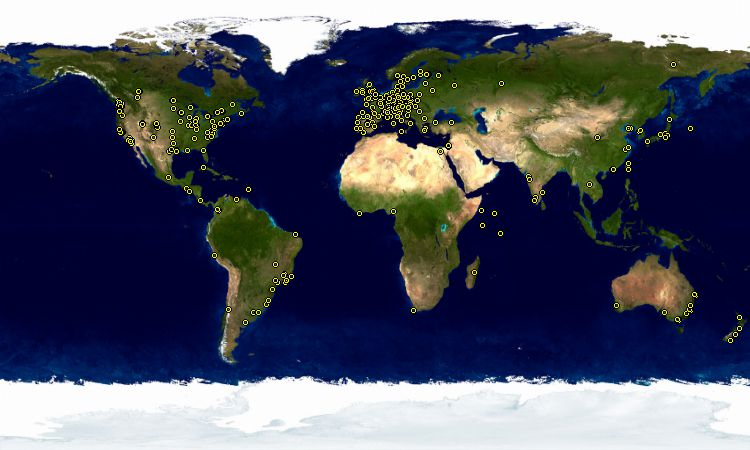
\includegraphics[width=8cm]{figs/developers-map}
%\caption{Map with the geographical location of Debian developers (as of 
%January 2015).}
%\label{fig:debian-map}
%\end{figure}

As another case, Mozilla's mission states that they want that ``people worldwide can be informed contributors and creators of the Web''\footnote{\url{https://www.mozilla.org/en-US/mission/}}, so information about virtual participation is useful to design a global strategy. This type of information can be used as well by companies to assess the interest on their FLOSS products in certain geographic areas, and as information helpful in opening new markets.

But getting this information is not easy in most cases, since there are little data sources to collect it. The goal of this paper is to show a methodology to obtain the geographic distribution of a FLOSS community by means of analyzing artifacts produced as side-product of the software development effort. Therefore data will be extracted from source code management systems (such as Git) and mailing list archives, and don't require the active collaboration of developers.

The structure of the rest of this paper starts with the presentation of related research.
% Section~\ref{sec:questions}
%contains the specific research questions that this paper targets. 
In Section~\ref{sec:methodology}, we detail the proposed methodology. Then we explain how we apply it to analyze the CloudStack project, as an illustrative case study (Section~\ref{sec:case-study}). Finally, some conclusions are drawn and future directions are discussed.


%-----------------------------------------------------------------------
%\section{Research questions}
%\label{sec:questions}
%
%\begin{enumerate}
%  \item
%
%  \item 
% 
%  \item 
%\end{enumerate}


%-----------------------------------------------------------------------
\section{Related research}
\label{sec:related}

The coordinated development of a software product by geographically distributed
teams has been a matter of study since the late 1990s~\cite{carmel1999global}.
The specific case of FLOSS communities has been considered in several cases~\cite{german2003gnome,engelhardt2009geographic,von2010geographic}, even with some attention to regions where FLOSS development is rare, such as Africa~\cite{ouattara2013open}.

Some of these efforts tried to estimate the location of the global FLOSS development community, such as the study of the geographical data obtained from the accounts of over one million registered users at SourceForge~\cite{robles2006geographic,gonzalez2008geographic}. In other cases, massive surveys were performed~\cite{ghosh2002free,david2008community}. Some of those asked for the country of origin and the current country of residence, in order to find developer migration patterns, finding how talent is attracted by the United States from all over the world~\cite{ghosh2002free}.

The target for this paper is not to obtain an statistical estimate of the global FLOSS community, but to obtain a picture as accurate as possible of the community of a given project. Therefore, instead of performing massive surveys or analyzing software development platforms with many projects, we target project-specific tools. A similar approach can be found in Bird et al. who have examined how two large FLOSS projects perform their work in a distributed manner~\cite{bird2012examining}. Related to the methods used in this paper, Tang et al. propose a set of 
techniques for identifying the country origin of mailing list participants~\cite{tang2009techniques}, which they use to perform a case study on the impact of global participation on mailing lists communications in FLOSS projects~\cite{tang2009case}.

%-----------------------------------------------------------------------
\section{Methodology}
\label{sec:methodology}

The analysis we propose is based on the traces left by developers in the Git repositories and mailing lists, and it can be easily extended to other data sources which log some geographical information.

%The results are based on the analysis of the Git repositories. Git is a
%distributed source code management system tool that allow developers to work
%in their own servers. Those changes to the source code, named as commits, can be
%later \emph{merged} or sent for a \emph{code review} process within the community.

In the specific case of Git, each commit includes as a part of its metadata some geographical information: a timezone. It is set according to the timezone obtained from the configuration of the computer where the commit took place, usually the one of the committer. And it is kept as the commit is merged in the main code base of the project. In the case of mailing lists, similar information is maintained in the message headers referring to dates. In particular, one of them keeps the timezone of the machine originating the message, usually that of the developer (or one configured with its timezone of residence).
%Those local commits that are later merged into the main branch, also named as \emph{master}.
%And 
%% Threats to validity: cherry pick, local setup of the timezone in the laptops,
%%                      people working around the world.

To obtain and use this information, we follow the following four steps:

\begin{enumerate}
\item Identification of data sources. This process needs of the understanding of the infrastructure used by the community or project to analyze. In FLOSS communities, the required information is typically accessible publicly. Since we focus on the development community, the relevant repositories are source code Git repositories, and development mailing lists.

\item Extraction of information from data sources. The data process extraction
is done with \emph{CVSAnalY}\footnote{\url{https://github.com/MetricsGrimoire/CVSAnalY}} (for Git) and \emph{MLStats}\footnote{\url{https://github.com/MetricsGrimoire/MailingListStats}} (for mailing lists), two FLOSS data extraction tools that store the information they retrieve in a MySQL/MariaDB database. It is part of the \emph{Metrics Grimoire toolset}\footnote{\url{https://github.com/MetricsGrimoire}}, built and maintained by our team.
%link to the tools for usual bla bla from IJOSSP.

\item Analysis of the dataset. Given the amount of information provided by CVSAnalY and MLStats, and that not all of it is needed for this analysis, several filters can be applied before starting the analysis. In the case of Git, we ignore \emph{merge} commits were ignored, and commits performed by bots: merges commits are in most cases performed automatically, or are not directly reflecting changes to the code, and bots do not directly correspond to the activity of a human. In the case of mailing lists, we ignore messages by bots, for the same reasons.

\item Timezone analysis. We use \emph{GrimoireLib}\footnote{\url{https://github.com/VizGrimoire/GrimoireLib/}}, a library specialized in the analysis of information organized in SQL databases produced by \emph{Metrics Grimoire tools}. This library provides a framework to deal with all of the resultant databases supporting the use of the output of \emph{CVSAnalY} and \emph{MLStats}. For our purposes, some new code was developed to perform the timezone analysis. It groups activities depending on the specified timezone, as a time difference from GMT, in integer hours (non-integer time zones, such as GMT+5:30, used in India, are rounded to their floor integer).

\end{enumerate}


%-----------------------------------------------------------------------
\section{Case Study: CloudStack}
\label{sec:case-study}

The CloudStack project\footnote{\url{http://cloudstack.apache.org/}} is a FLOSS project under the umbrella of the Apache Software Foundation. Its main goal is to provide easy deployment and management of large networks of virtual machines. This project provides infrastructure as a service (IaaS) highly available and scalable.

The first traces of information about CloudStack activity in their Git repositories start in August 2010. These repositories hold, at the end of 2015, close to 40,000 commits and 300 different developers with at least one commit of activity during these years.

The methodology presented in the previous section was applied to all these repositories.

%CloudStack is a project that was born in California; however, nowadays it has
%a global community.

% as it can be seen from the fact that a company contributing
%to the project has Indian professional developers working on the project.

%talk about the community origins of the CloudStack project. Where
%the project originated (in California) and who works on it now (the Indian
%guys from XX company)

%-----------------------------------------------------------------------
%\section{Results}
%\label{sec:results}

%In this section we show the result of applying the aforementioned methodology
%on our case study, CloudStack. 
We apply our methodology to two different
sources from CloudStack: Git source code management (SCM) repositories and mailing lists archives (MLs). From SCM repositories we can obtain geographic information about how distributed the team of software developers is. Data from MLs provides information about the development community in general, including contributors to activities different than coding.

\subsection{Analysis of SCM}

%First, the analysis of the \texttt{git} repository, the SCM
%system in use in CloudStack, will we presented. 

We have grouped commits on a yearly basis, and showed the results graphically for number of distinct authors and number of commits for each period. The number of distinct authors is a good proxy of the number of developers working on the project, while the number of commits gives an idea of the overall development activity.

Figure~\ref{fig:2010-scm} shows the results for the early phases of the
project (year 2010). The horizontal axis references the detected time-zone
relative to UTC. As it can be observed from the chart for authors, there is just one developer in UTC+0 (the timezone for UK, Ireland and Portugal), and three in UTC+5 (India). Almost all developers are located in timezones corresponding to the U.S. West Coast (UTC-7 and UTC-8, for Winter and Summer time), with some very likely in the U.S. East Coast (UTC-5 and UTC-4), although these timezones are shared with some countries in South America.

The chart for commits is even more revealing, which most of the activity clearly focused on the U.S. West Coast: so much, that the contributions from other regions are almost negligible.

In summary, CloudStack was in 2010 a project that had developers from several regions, but the main development activity was clearly concentrated in the U.S. West Coast.

\begin{figure}[!h]
\centering
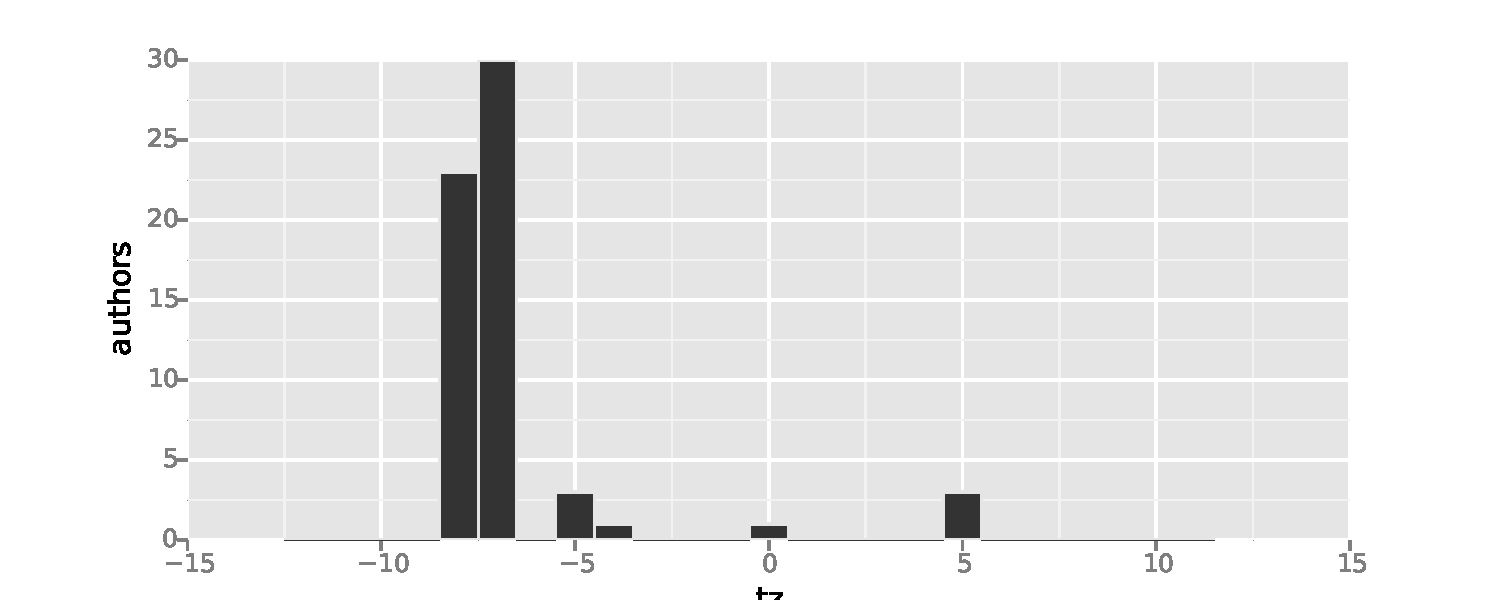
\includegraphics[width=6.9cm]{figs/cloudstack/tz-scm-authors-2010.pdf}
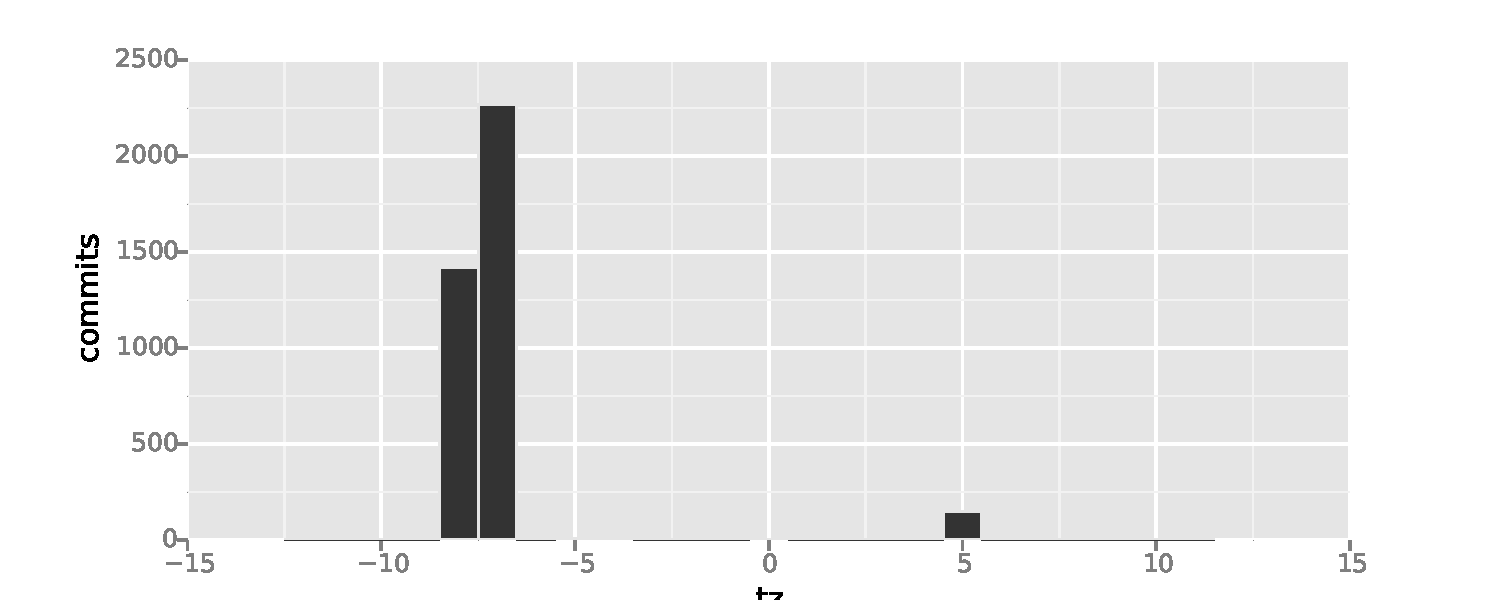
\includegraphics[width=6.9cm]{figs/cloudstack/tz-scm-commits-2010.pdf}
\caption{Time-zone analysis for authors (top) and commits (bottom) for
the CloudStack Git repositories (2010).}
\label{fig:2010-scm}
\end{figure}

Figure~\ref{fig:2014-scm} shows the same analysis for CloudStack Git repositories during 2014. As we can see from the authors chart, their number increased significantly in those four years. In addition, the project was more geographically distributed. Now we can observe authors from all America time zones, although the West Coast is still predominant. The three European timezones (UTC+0 to UTC+2) have all over 20 developers, and India (UTC+5) has the maximum number
of authors, 55. Developers from other Asian areas, or from Australia, are marginally present too (UTC+7 to UTC+10).

If we observe the commits chart in the same Figure~\ref{fig:2014-scm}, we see that CloudStack development activity is performed in three regions: the U.S. (with a peak in the West), Europe (with a peak in Eastern Europe, UTC+2) and India (UTC+5).

\begin{figure}[!h]
\centering
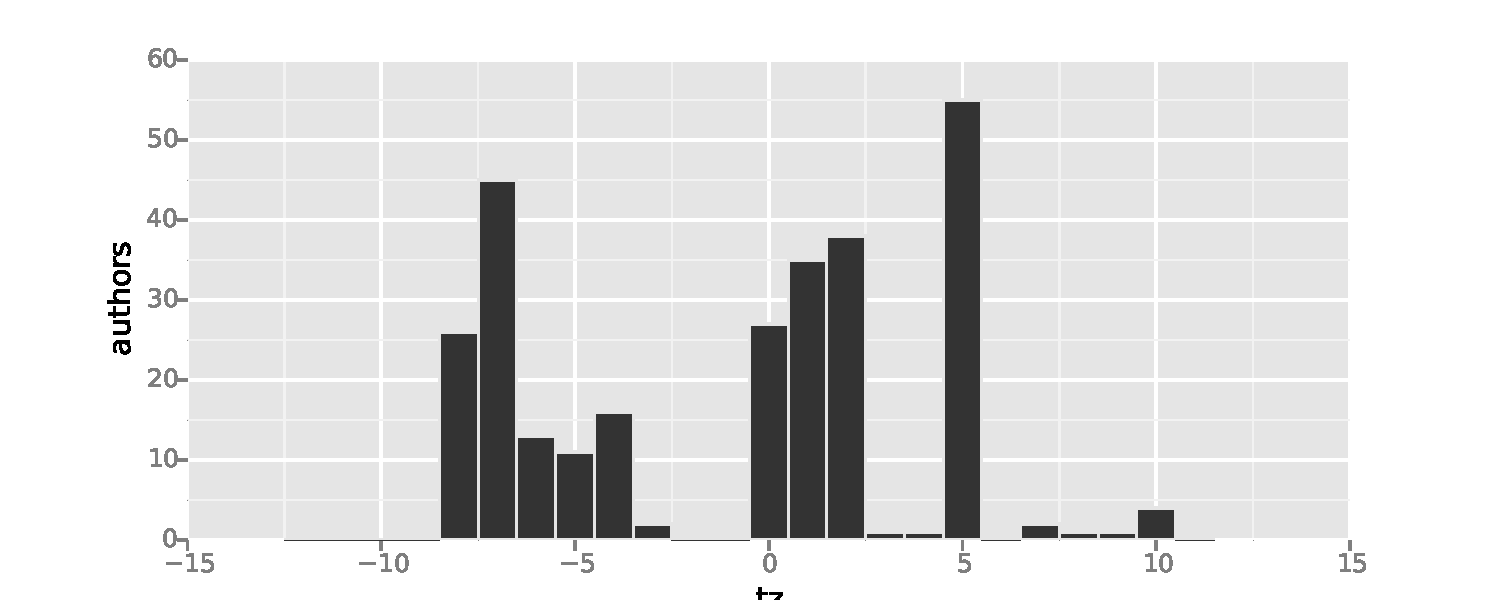
\includegraphics[width=6.9cm]{figs/cloudstack/tz-scm-authors-2014.pdf}
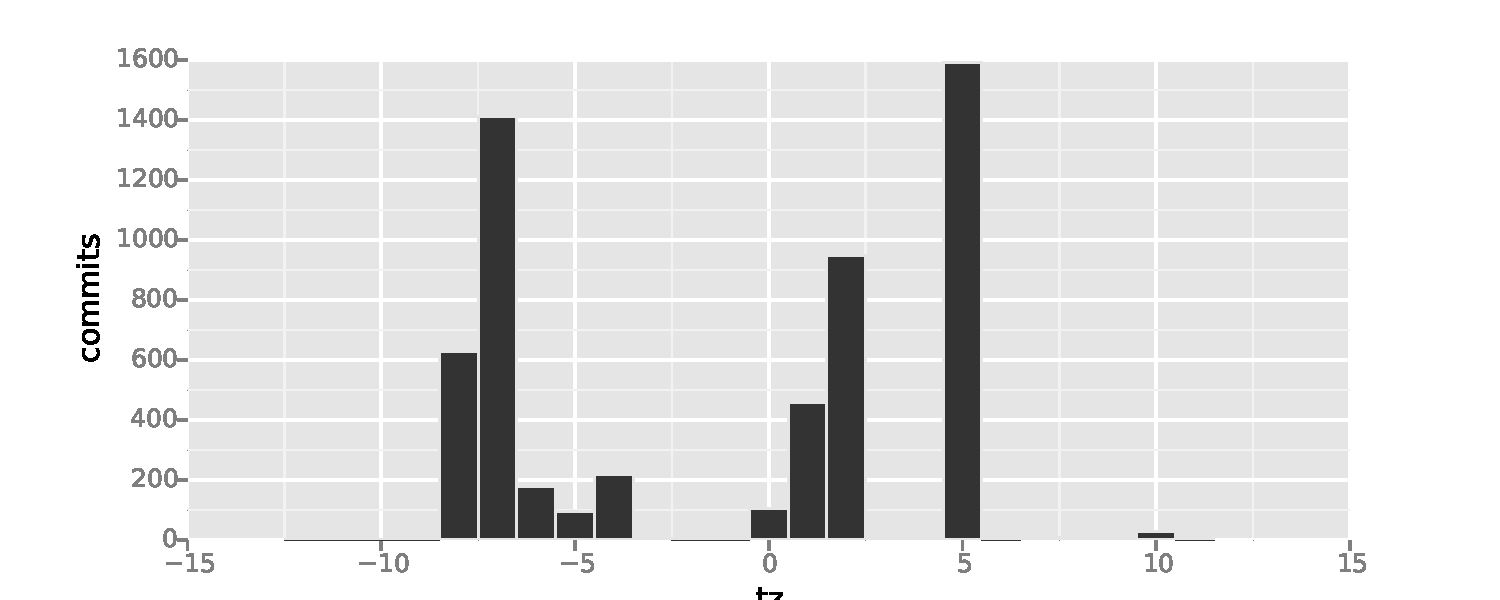
\includegraphics[width=6.9cm]{figs/cloudstack/tz-scm-commits-2014.pdf}
\caption{Time-zone analysis for authors (top) and commits (bottom) for
the CloudStack Git repositories (2014).}
\label{fig:2014-scm}
\end{figure}


\subsection{Analysis of MLs}

Figure~\ref{fig:2012-mls} shows the results for the analysis of the
CloudStack MLs for the year 2012. The vertical axis in the authors chart represents provides the number of different authors, while for the messages chart it corresponds to number of messages. MLs in 2012 already showed a global distribution
of participants of the CloudStack project, hinting that authorship and activity
in MLs possibly precedes development activity. However, there are
two interesting aspects that require a specific analysis by themselves: the cases of UTC+0 and UTC+8. UTC+0 includes authors and activity from countries
such as UK, Ireland or Portugal, but as well all those who configure their timezone as ``GMT'' in their mail clients, such as for example many frequent travelers do. Therefore, the data for UTC+0 has to be considered with some precaution. In the case of UTC+8, which corresponds to China, Southeast Asia and Australia's Western Standard Time, among other territories, it is strange how there is a large number of authors, but few messages have been sent. This very corresponds to a much lower participation per person than in other regions.

\begin{figure}[!h]
\centering
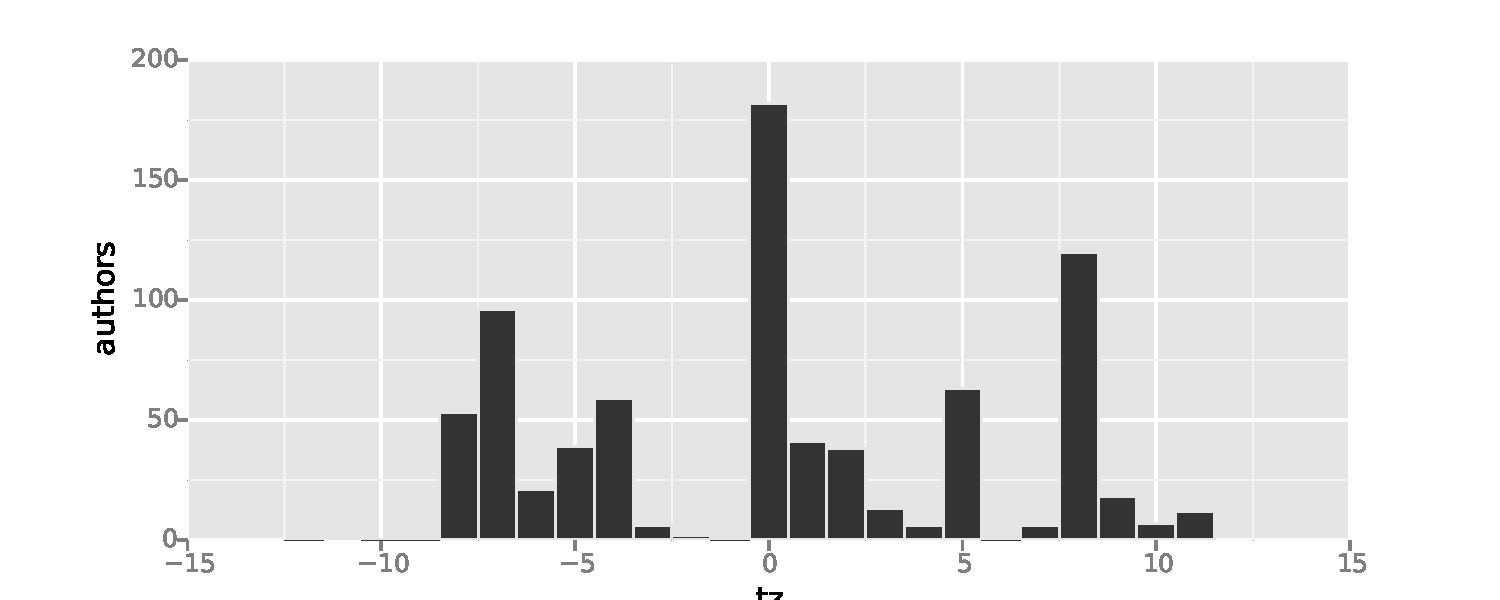
\includegraphics[width=6.9cm]{figs/cloudstack/tz-mls-authors-2012.pdf}
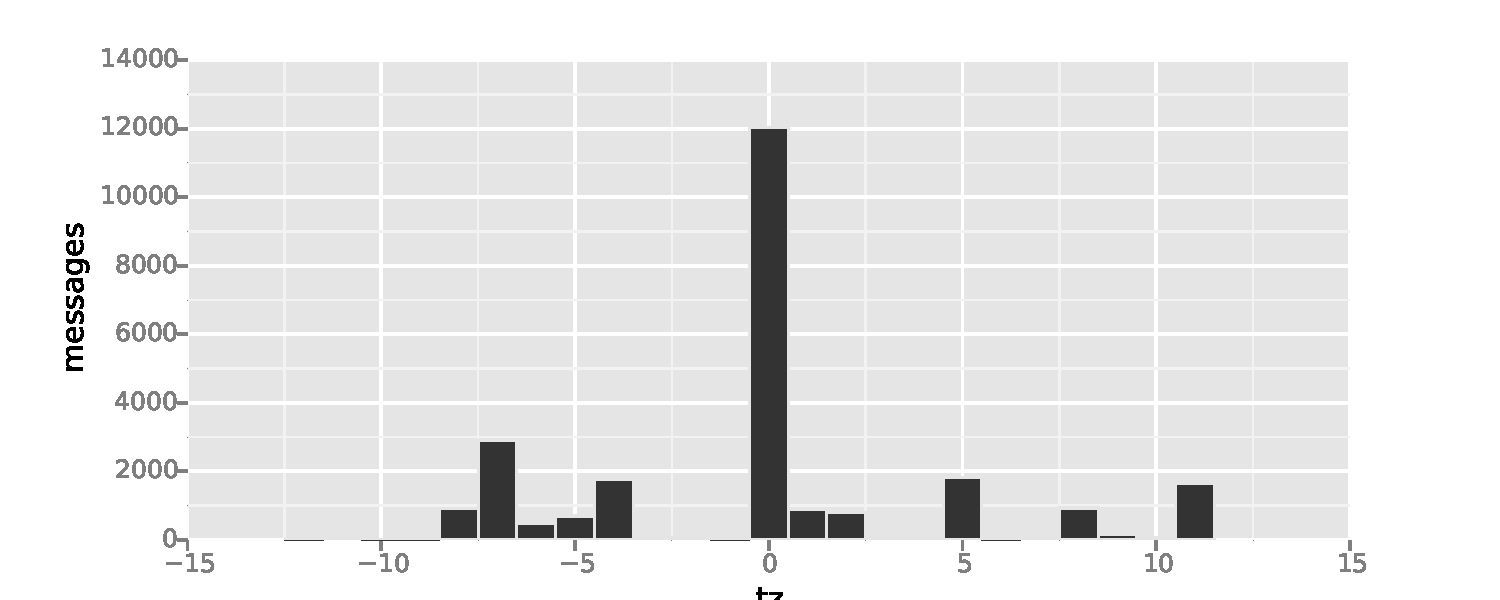
\includegraphics[width=6.9cm]{figs/cloudstack/tz-mls-messages-2012.pdf}
\caption{Time-zone analysis for authors (top) and messages (bottom) for
the CloudStack development mailing list archives (2012).}
\label{fig:2012-mls}
\end{figure}

Figure~\ref{fig:2014-mls} shows the same analysis for MLs during 2014. Again, UTC+0 is the most significant timezone, which heavily biases results, thus limiting the possibility of performing a proper analysis.

\begin{figure}[!h]
\centering
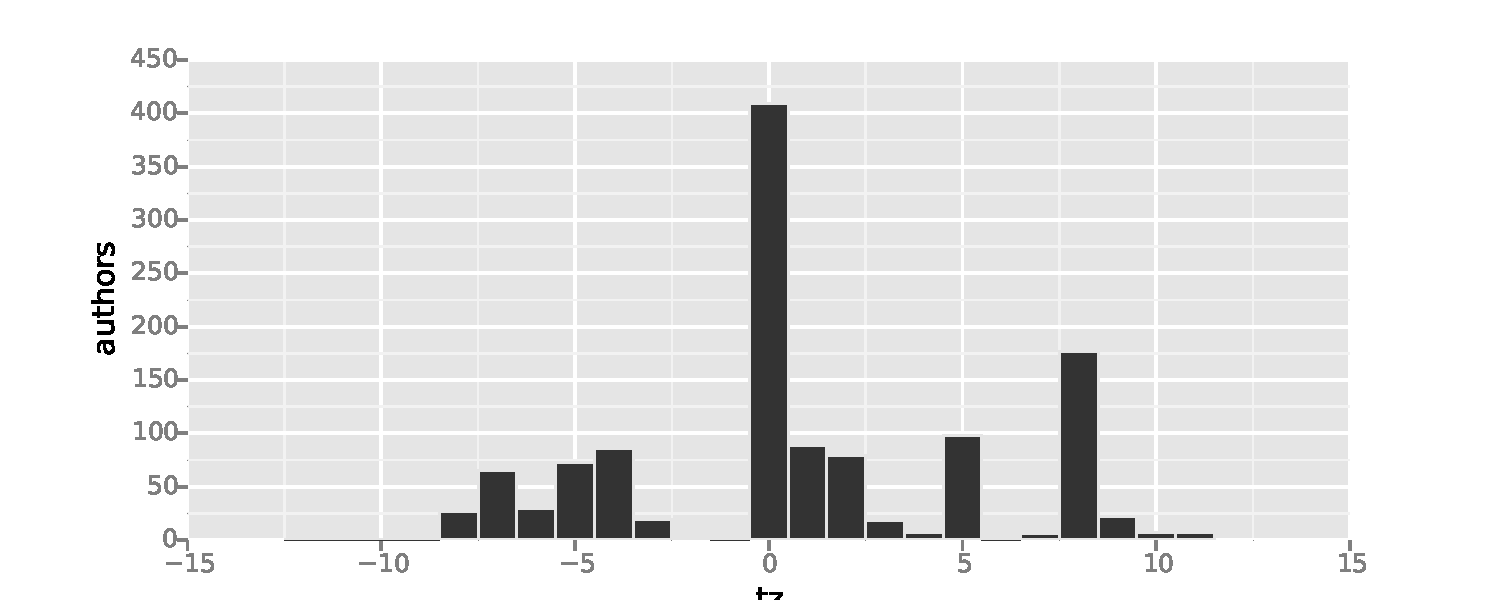
\includegraphics[width=6.9cm]{figs/cloudstack/tz-mls-authors-2014.pdf}
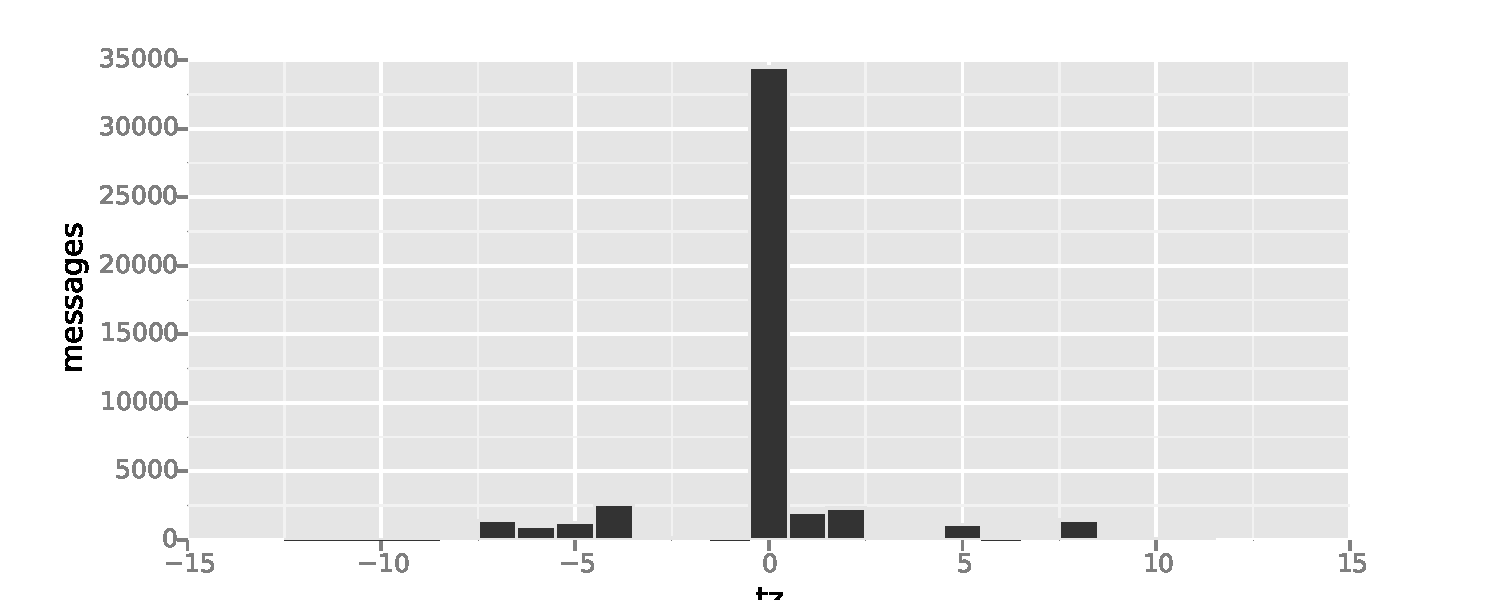
\includegraphics[width=6.9cm]{figs/cloudstack/tz-mls-messages-2014.pdf}
\caption{Time-zone analysis for authors (top) and messages (bottom) for
the CloudStack development mailing list archives (2014).}
\label{fig:2014-mls}
\end{figure}


%-----------------------------------------------------------------------
\section{Discussion and conclusions}
\label{sec:discussion}

We have shown how the proposed methodology allows for the determination of the main geographical areas with activity related to development. In the case of CloudStack we could find out how it started in a certain region, and later expanded to 
be globally distributed.

The methodology can be fully automated, and it uses as the basis for its analysis data that is in general available or can easily be obtained.

However, there are some limitations:

\begin{enumerate}

  \item Some regions have a different time zone during Winter and Summer. This can mangle the results, at least visually.

  \item The nature of timezones, comprising several regions, makes it impossible to know to what specific zone belongs a developer. For example the Central European time zone includes from Spain to Poland in Europe, but many African countries as well.

  \item The UTC+0 configuration problem in email clients may cause a severe 
\emph{bias} for this time zone, as it has been shown in the analysis of the
MLs in CloudStack.

  \item Sometimes, obtaining the data for the mailing
list analysis is not straightforward as the archives only store the server
date. To perform the analysis correctly, the time and time zone data in the original messages has to be preserved, and it not always is.

\end{enumerate}

In summary, we have presented a methodology that can be used to measure
the geographic distributed of a FLOSS project. It is based on data that
is in general publicly available, as a side-product of software development processes. With the help of a case study, we have explored how we can infer 
information about the geographic dispersion of contributors to the project,
and how it changes over time.

As future work we plan to apply this methodology to other projects to find
out if different patterns can be found.

%-----------------------------------------------------------------------
\section*{Acknowledgments}

The work of Jesus Gonzalez-Barahona and Gregorio Robles has been funded in part by the Spanish Gov. under SobreVision (TIN2014-59400-R) and by Comunidad de Madrid under eMadrid (S2013/ICE-2715). Daniel Izquierdo-Cortazar is supported by the Spanish Gov., Torres Quevedo grant (PTQ-12-05577). All three authors are supported in part by the European Comission, under Seneca, H2020 Program (H2020-MSCA-ITN-2014-642954).



%
% The following two commands are all you need in the
% initial runs of your .tex file to
% produce the bibliography for the citations in your paper.
\bibliographystyle{plain}
\bibliography{biblio}  % sigproc.bib is the name of the Bibliography in this case
% You must have a proper ".bib" file
%  and remember to run:
% latex bibtex latex latex
% to resolve all references
%
% ACM needs 'a single self-contained file'!
%
%APPENDICES are optional
%\balancecolumns

\end{document}
